\section{研究目标}
\begin{enumerate}[leftmargin=0em, label=(\theenumi)]
%\setlength{\leftmargin}{0em}
\setlength{\itemindent}{4em}
\setlength{\labelsep}{0em}
\setlength{\labelwidth}{2em}
\setlength{\parsep}{0em}
\setlength{\itemsep}{0em}
\setlength{\topsep}{0em}
%\begin{enumerate}[leftmargin=0em, listparindent=2em, parsep=0em, topsep=0em, label=(\theenumi)]
%\setlength{\itemindent}{4em}
%\setlength{\labelsep}{0em}
%\setlength{\labelwidth}{2em}
%\setlength{\parsep}{0em}
%\setlength{\itemsep}{0em}
%\setlength{\topsep}{0em}
  \item 为满足行为交互实验过程中仿生机器鼠动作实时性和快速性要求,观察生物鼠在实验场景中的典型动作,提取其在交互行为中的动作特点,并据此设计、规划仿生机器鼠的仿鼠动作。
  \item 为满足交互实验仿真需求,利用计算机系统搭建一套仿生机器鼠行为交互实验的专用仿真平台,完成仿生机器鼠仿鼠行为驱动程序编写。\label{item_target_2}
  \item 针对生物鼠行为的快速性、个体差异及其对环境渐进适应的特性,提出一套基于强化学习的仿生机器鼠行为控制方法,使机器鼠与生物鼠进行有效交互,并利用\ref{item_target_2}中搭建的仿真平台进行验证。
\end{enumerate}

\begin{figure}[htbp]
  %\vspace{13pt} % 调整图片与上文的垂直距离
  \centering
  \subfigure[机器鼠营救被困的生物鼠]{
  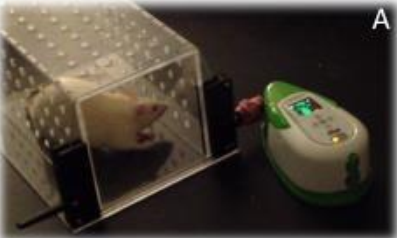
\includegraphics[width=0.4\linewidth, height=0.18\linewidth]{images/ch01/rescure/a.png} \label{figure_rescure_a}
  }
  \subfigure[生物鼠嗅探机器鼠]{
  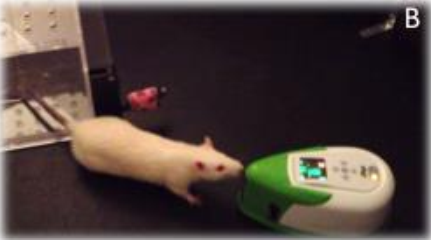
\includegraphics[width=0.35\linewidth, height=0.18\linewidth]{images/ch01/rescure/b.png} \label{figure_rescure_b}
  }
  \subfigure[生物鼠发现机器鼠被困]{
  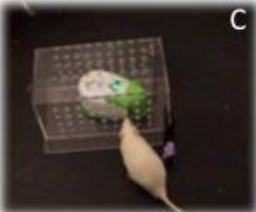
\includegraphics[width=0.23\linewidth, height=0.18\linewidth]{images/ch01/rescure/c.png} \label{figure_rescure_c}
  }
  \subfigure[生物鼠走向机关]{
  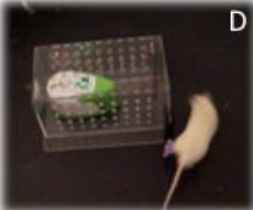
\includegraphics[width=0.23\linewidth, height=0.18\linewidth]{images/ch01/rescure/d.png} \label{figure_rescure_d}
  }
  \subfigure[生物鼠按下机关]{
  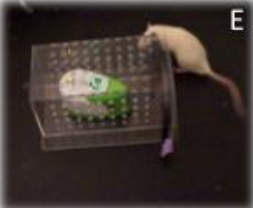
\includegraphics[width=0.23\linewidth, height=0.18\linewidth]{images/ch01/rescure/e.png} \label{figure_rescure_e}
  }
  \subfigure[生物鼠与机器鼠在笼中交互]{
  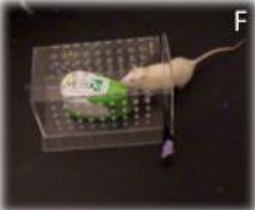
\includegraphics[width=0.23\linewidth, height=0.18\linewidth]{images/ch01/rescure/f.png} \label{figure_rescure_f}
  }
  \caption{生物鼠营救被困的“有作用的”机器鼠\cite{quinnWhenRatsRescue2018}}\label{figure_rescure}
\end{figure} 